% Figure snippets for main.tex. Embed these inline.

\begin{figure}[htbp]
\centering
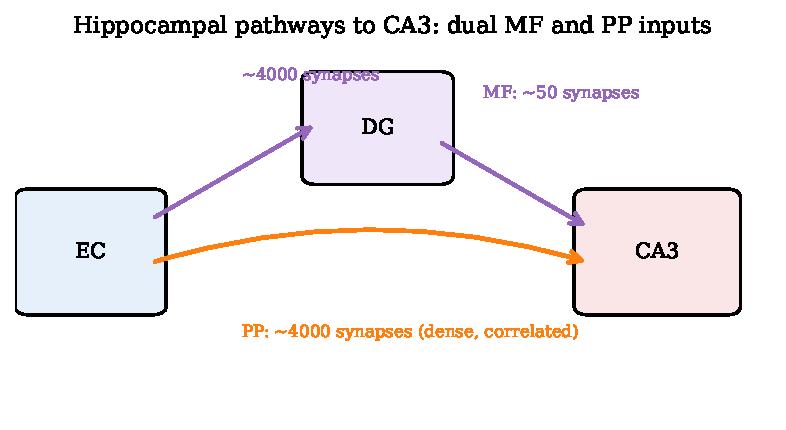
\includegraphics[width=0.88\textwidth]{figures/fig_pathways.pdf}
\caption{Schematic of hippocampal pathways to CA3. Entorhinal cortex (EC)
projects directly to CA3 through the perforant path (PP, dense, approximately
4000 synapses per CA3 pyramidal cell), and indirectly via the dentate gyrus
(DG) and its mossy fibers (MF, sparse, approximately 50 granule cell inputs
per CA3 pyramidal cell). Anatomical values are taken from the extraction.}
\label{fig:pathways}
\end{figure}

\begin{figure}[htbp]
\centering
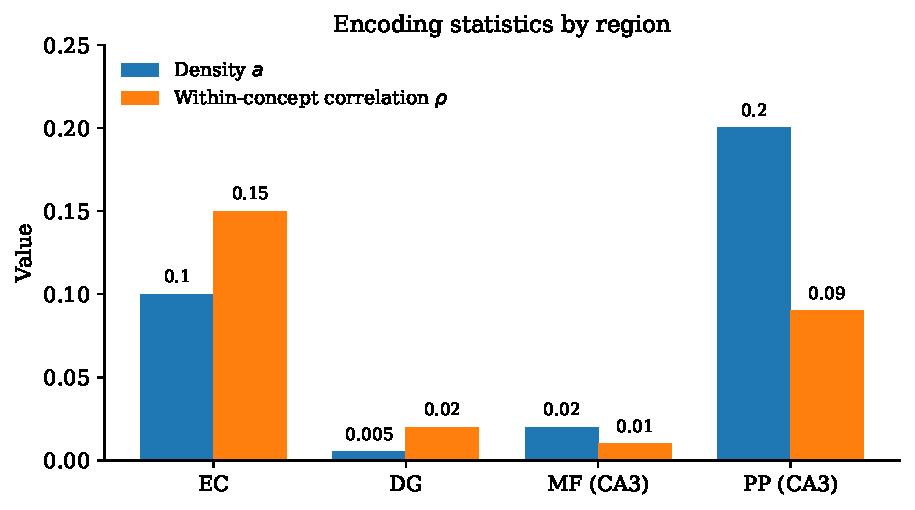
\includegraphics[width=0.78\textwidth]{figures/fig_density_correlation.pdf}
\caption{Encoding statistics across regions used in the model. Densities $a$
and within-concept correlations $\rho$ are those imposed by the winners-take-all
mechanism and measured from the FashionMNIST encodings: $a_{\mathrm{EC}} = 0.1$,
$a_{\mathrm{DG}} = 0.005$, $a_{\mathrm{MF}} = 0.02$, $a_{\mathrm{PP}} = 0.2$ and
$\rho_{\mathrm{EC}} = 0.15$, $\rho_{\mathrm{DG}} = 0.02$,
$\rho_{\mathrm{MF}} = 0.01$, $\rho_{\mathrm{PP}} = 0.09$. MF encodings are the
sparsest and least correlated; PP encodings are the densest and most
correlated.}
\label{fig:density_correlation}
\end{figure}

\begin{figure}[htbp]
\centering
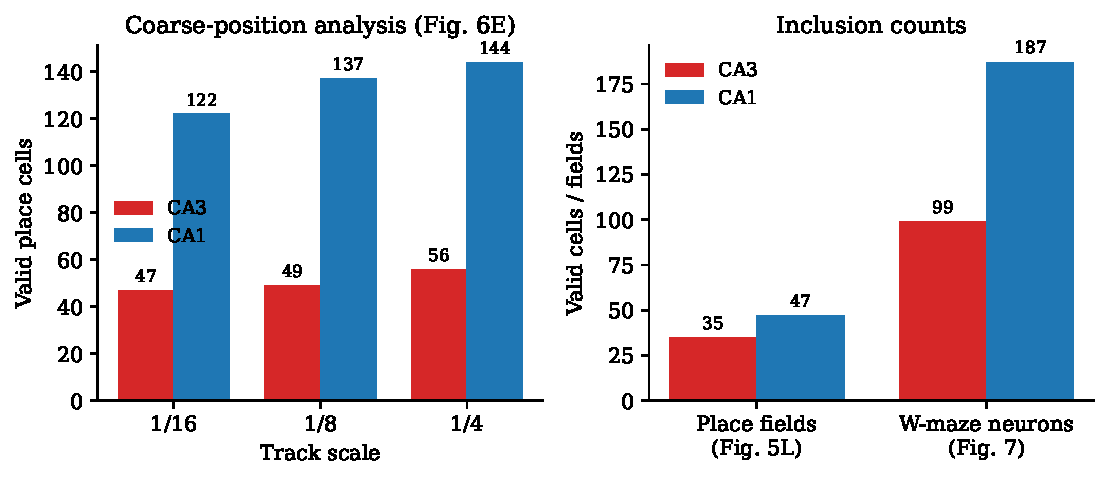
\includegraphics[width=0.95\textwidth]{figures/fig_valid_cells.pdf}
\caption{Numbers of valid cells and fields passing the inclusion criteria
described in Methods. Left: coarse-position analysis at track scales
$1/16$, $1/8$, $1/4$ yields 47, 49 and 56 valid CA3 place cells and 122, 137
and 144 valid CA1 place cells, respectively. Right: the fine-scale place
field analysis yields 35 valid CA3 fields and 47 valid CA1 fields, while the
W-maze task yields 99 valid CA3 neurons and 187 valid CA1 neurons.}
\label{fig:valid_cells}
\end{figure}

\begin{figure}[htbp]
\centering
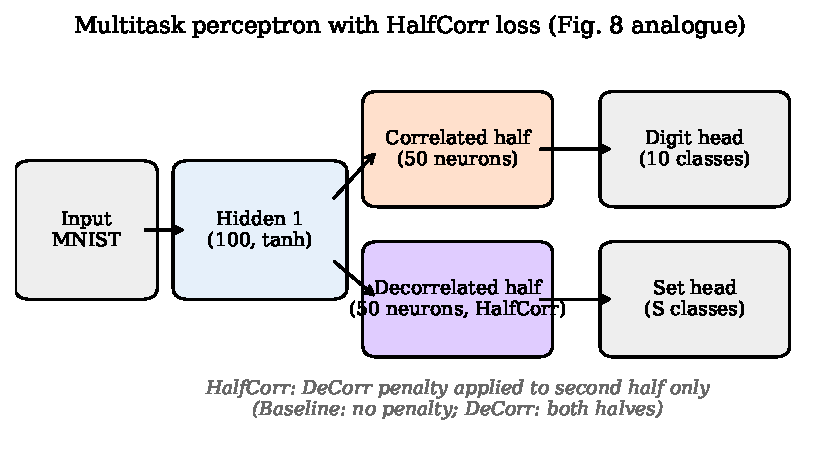
\includegraphics[width=0.90\textwidth]{figures/fig_ml_schematic.pdf}
\caption{Multitask multilayer perceptron architecture. Two fully connected
hidden layers of 100 tanh units feed two softmax output heads, one for digit
classification and one for set identification. The HalfCorr loss applies the
DeCorr penalty only to the second half of the final hidden layer, yielding
a correlated half (PP-like, orange) and a decorrelated half (MF-like,
purple). The DeCorr baseline applies the penalty to all neurons, while the
baseline condition applies no penalty.}
\label{fig:ml_schematic}
\end{figure}

\begin{figure}[htbp]
\centering
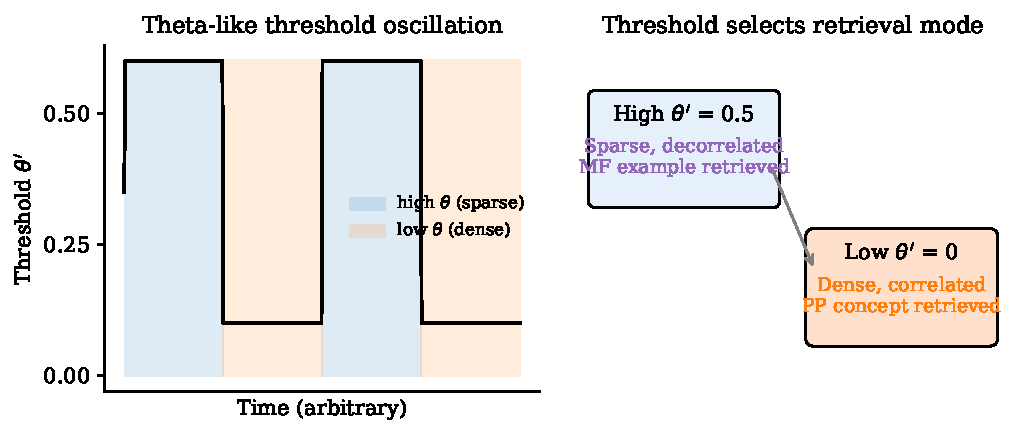
\includegraphics[width=0.95\textwidth]{figures/fig_retrieval_schematic.pdf}
\caption{Threshold control of retrieval in the Hopfield-like CA3 model.
Left: a theta-like oscillation in the rescaled activity threshold alternates
between a high value ($\theta' = 0.5$) that favors MF example retrieval and
a low value ($\theta' = 0$) that favors PP concept retrieval. Right: at high
threshold the network retrieves the sparse, decorrelated MF representation
of the cued memory; at low threshold, a dense, correlated PP representation
emerges that merges examples along shared features.}
\label{fig:retrieval_schematic}
\end{figure}
